\documentclass[conference]{IEEEtran}
\pdfminorversion=7

\usepackage{algorithm}
\usepackage{algpseudocode}
\usepackage{amsthm}
\usepackage{booktabs,tabularx}
\usepackage{cite,url}
\usepackage{amsmath,amssymb,amsfonts}
%\usepackage{algorithmic}
\usepackage{graphicx}
\usepackage{textcomp}
\usepackage{xcolor}
\usepackage{comment}
\usepackage{subcaption}
\usepackage{siunitx}
\usepackage{colortbl} 
\usepackage{multirow}
\usepackage[hidelinks]{hyperref}

\setlength{\textfloatsep}{6pt plus 1pt minus 2pt}
\setlength{\floatsep}{6pt plus 1pt minus 2pt}
\setlength{\intextsep}{6pt plus 1pt minus 2pt}
\setlength{\abovecaptionskip}{3pt}

\newtheorem{remark}{Remark}
\newtheorem{definition}{Definition}
\newtheorem{theorem}{Theorem}

\begin{document}

\title{TRAPS: Risk-Aware One-Sided Admission Indexing for High-Cost Point Queries}
\author{
  Yadi Wen, Yaxuan Wang, Yujie Xu, Yaling Ren, Dan Yu, Rong Du, Yue Fu, Yongle Chen\\
  \IEEEauthorblockA{
Shanxi Key Laboratory of Industrial Internet Security, Taiyuan University of Technology, China\\
Emails: \{2023005322, 2023005749, 2024002194, 2023006489\}@link.tyut.edu.cn,\\ \{yudan, durong, fuyue, chenyongle\}@tyut.edu.cn
  }
}
\maketitle

\begin{abstract}
We study admission indexing for high-cost point queries. Password verification is our case study: a frontend should reject definite invalid credential pairs before they invoke Argon2id/PBKDF2, while never dropping represented valid credentials. TRAPS separates routing from correctness. A stable learning and risk oracle assigns attempts to regions, and each region is backed by a keyed approximate-membership substrate or compatible keyed tag fingerprint; the backend remains the only accepting authority. TRAPS uses a capped water-filling allocator for regional residual-forward budgets, records backend-confirmed false positives in an exact replay cache, and preserves one-sidedness through stable features and versioned migration. Seeded controlled frontiers, shift grids, dynamic fallback, LANL-conditioned replay, keyed-tag baselines, scale/update, and bounded-worker queueing show the trade-off: keyed tag fingerprints give strong uniform collision bounds, while AMQ-backed TRAPS provides risk-aware residual-channel allocation without placing learning on the authentication-correctness path.
%\keywords{Password authentication, Learned Bloom filter, Credential-flooding defense, Application-layer denial-of-service, Adaptive false-positive control, Capacity-aware pre-screening}

\end{abstract}

\section{Introduction}

Password verification is a stream of high-cost point queries: each submitted account--password tuple asks whether an expensive backend hash should run. Modern deployments deliberately use costly PBKDF2, scrypt, or Argon2id parameters~\cite{nist_sp800_63b_2017}; this protects stored passwords, but makes invalid online attempts nearly as expensive as legitimate logins.

\paragraph{Admission-index design problem}
Let \(K_t\) be represented credential keys at epoch \(t\). An admission index returns \textsc{reject} or \textsc{forward}; it is one-sided if every \(q\in K_t\) is always forwarded. Given memory, update limits, risk regions, and a shifting invalid stream, the physical-design objective is to minimize invalid forwards to the backend subject to one-sided correctness and per-region residual-forward budgets. Exact keyed fingerprints and AMQs such as Bloom filters~\cite{broder2004network} can serve as lightweight pre-verifiers, but a single global budget is risk-agnostic: known-password and chosen-password traffic can steer load toward regions where deterministic false positives amplify backend work.

TRAPS is a first-party learned admission layer that keeps learning off the authentication-correctness path. A stable risk oracle routes attempts into regions; a region-local substrate decides only whether to forward to the backend. Learning affects resource allocation rather than authentication correctness: it changes which residual channel and capacity budget a query sees. The oracle never accepts a credential and never rejects a represented credential by itself. Correctness follows from stable features, atomic insertion, and versioned epoch migration; oracle errors only change efficiency.

The abstraction is substrate-agnostic. Exact keyed tags are the strongest fast-verifier point when account-local tag storage is acceptable, while AMQ-backed TRAPS addresses the approximate-membership regime where residual false forwards must be allocated across regions. TRAPS adds capped region allocation, which prevents any routed region from becoming an unbounded steering target, and an exact replay cache that suppresses backend-confirmed false positives. Our Argon2 prototype evaluates controlled credential floods, shift/fallback behavior, LANL status-outcome replay, invalid-heavy trace-conditioned replay, update cost, queueing, and ablations.

\paragraph{Design scope}
The paper evaluates two complementary regimes. Exact keyed tags provide the measured fast-verifier frontier when account-local tag storage is acceptable. AMQ-backed TRAPS studies how to distribute an unavoidable residual false-forward channel across risk regions, replay discoveries, and rebuild epochs. Distribution shift is handled through next-epoch capacity updates, dual-query migration, and drift fallback.

\paragraph{Contributions}
\begin{itemize}
    \item We formulate password-verification floods as a risk-aware one-sided admission-index physical-design problem with memory, update, and regional residual-forward budgets.
    \item We give a capped water-filling allocator with a feasibility certificate and closed-form KKT solution for regional residual channels.
    \item We present AMQ-backed TRAPS: stable learned routing, exact replay suppression, and versioned migration that preserve one-sidedness.
    \item We define a substrate interface for AMQs and keyed fingerprints, including exact-tag rows as the fast-verifier frontier.
    \item We evaluate credential-flood, drift/fallback, LANL-conditioned replay, update, queueing, and ablation workloads.
\end{itemize}

\section{Building Blocks}
\label{sec:blocks}

This section defines the mechanisms used by TRAPS. The concrete known-password and chosen-password attack models are introduced in Section~\ref{sec:threat-model}.

\paragraph{Notation}
Let \(S\) be the active credential set and \(N:=|S|\). A credential consists of a username, password, account salt, password-version number, and stable credential metadata. We write \(H\) for the expensive backend password-verification function and \(h\) for a lightweight prehash. A \emph{member} query is a correct login attempt for an active credential. A \emph{non-member} query is an incorrect attempt relative to the active credential set.

TRAPS partitions credential attempts into \(r\) regions. Let \(S_j\subseteq S\) be the set of represented valid credentials assigned to region \(j\), and let \(N_j:=|S_j|\). For sizing, \(\bar N_j\) denotes the provisioned occupancy of region \(j\).

\subsection{Learning-Assisted Indexing Interface}

TRAPS separates routing from membership. The learning and risk oracle maps an attempt to a region, while a region-local fast-verification substrate decides whether the attempt should be escalated to the backend.

A region-local substrate exposes the interface
\[
\mathcal I_{e,j}.\mathsf{Query}(t)\in\{\mathsf{neg},\mathsf{pos}\},
\]
where \(e\) is the epoch, \(j\) is the region, and \(t\) is a credential trapdoor. A negative result is locally rejected with the generic failure response. A positive result is only an escalation decision: the backend verifier \(H\) remains responsible for accepting or rejecting the login.

This interface can be implemented by AMQs, such as Bloom filters, Cuckoo filters, or quotient filters, or by exact keyed fingerprints. The security invariant is the same across substrates: represented valid credentials must not be locally dropped by the pre-screener.

\subsection{Two Membership Problems}

TRAPS separates two membership problems that are often conflated.

\paragraph{Credential membership}
The first problem is to test whether a submitted username--password pair is plausibly represented by the active credential set. This test must have one-sided correctness: a represented valid credential must not be locally rejected by the pre-screener.

Exact keyed fingerprints solve this problem directly. For example, a service may store a truncated keyed tag
\[
\theta_u
=
\operatorname{Trunc}_b
\left(
\operatorname{HMAC}_{K}
\left(
u\parallel pw\parallel s_u\parallel v_u
\right)
\right)
\]
and compare it before invoking \(H\). This is a strong baseline for uniform account-local fast verification.

A \(b\)-bit keyed tag has residual collision probability approximately \(2^{-b}\) per attempt. An optimally tuned Bloom filter with \(B\) bits per represented key has
\[
p_{\mathrm{BF}}(B)\approx \exp\!\left(-(\ln 2)^2B\right)=2^{-B\ln 2}.
\]
Thus, at the same nominal 16 bits per key, a tag targets about \(1.5\times10^{-5}\) residual forwards, while a Bloom filter targets about \(4.6\times10^{-4}\). This gap is a substrate property. TRAPS uses a regioned indexing layer to assign different residual forwarding budgets to different risk populations. Exact keyed fingerprints give the fast-verifier operating point; AMQs give a compact, centrally partitionable operating point that naturally supports region-wise memory allocation.

\paragraph{Risk membership}
The second problem is to identify whether an attempt belongs to a risky population, such as attempts using leaked or policy-denied passwords, or registrations that resemble chosen-password occupancy manipulation. This signal may be approximate. False positives can route an attempt into a stricter region, and false negatives leave some attack traffic in a less hardened region. Such signals must not directly accept or reject an existing credential at login.

TRAPS uses risk membership only for routing and hardening. Final authentication is still performed by the backend verifier, and valid-credential forwarding is protected by the credential-membership invariant.

\subsection{PRF Trapdoors}

Let \(\kappa\) be the security parameter, and let
\[
\mathsf{F}=\{f_K\}_{K\in\{0,1\}^{\kappa}}
\]
be an efficiently computable pseudorandom function with output domain \(\mathcal{T}\). For username \(u\), password \(pw\), salt \(s\), and epoch trapdoor key \(K_e^{\mathrm{td}}\), TRAPS derives the credential trapdoor
\[
t
=
f_{K_e^{\mathrm{td}}}
\left(
h(u,pw,s)
\right)
\in\mathcal{T}.
\]
The trapdoor is used only as the membership key for the fast-verification substrate. It is not exposed as a learning feature and does not determine authentication success.

At enrollment, \(s=s_u\) is the account salt. At login, the frontend uses \(s=s_u\) if the username exists in the edge directory and a dummy salt \(s=\bar{s}\) otherwise. Unknown usernames therefore follow the same logical trapdoor-generation path but query trapdoors that were never inserted.

\subsection{AMQ Credential Screening}

In our implementation, each region is backed by one or more Bloom filters~\cite{broder2004network}. Bloom filters are the measured AMQ substrate in this paper; Cuckoo, quotient, XOR, or fused filters can instantiate the same interface but are not separately evaluated here. A Bloom filter stores a set using a bit array and public hash functions. It has one-sided error: inserted items are never missed, while non-inserted items may query positive.

For a Bloom filter with \(n\) inserted items, \(m\) bits, and \(k\) hash functions, the standard false-positive approximation is
\[
\mathrm{FPR}_{\mathrm{BF}}(n,m,k)
=
\left(1-e^{-kn/m}\right)^k.
\]
With near-optimal hashing,
\[
k\approx \frac{m}{n}\ln 2.
\]
TRAPS provisions each region \(j\) with an effective residual forwarding probability \(\varepsilon_j\). A non-member attempt routed to region \(j\) reaches the backend with probability approximately \(\varepsilon_j\), before replay suppression is applied.

\subsection{Learning and Risk Oracle}

TRAPS uses learning only to partition attempts into regions. Let
\[
x=\phi_e(u,pw,\sigma)
\]
be an epoch-stable feature vector, where \(\sigma\) denotes stable account or credential metadata. The risk oracle
\[
\mathcal{O}_e(x)\in[0,1)
\]
may combine learned scores with risk-membership probes such as known-password-list membership or registration-side chosen-password markers. Thresholds
\[
0=\tau_0<\tau_1<\cdots<\tau_r=1
\]
define the routing rule
\[
\pi_e(u,pw,\sigma)=j
\iff
\tau_{j-1}\le \mathcal{O}_e(\phi_e(u,pw,\sigma))<\tau_j.
\]

The oracle differs from learned Bloom filters that predict set membership~\cite{Mitzenmacher2018NeurIPS}: it predicts a resource region, while membership remains a keyed substrate query. Model errors can place traffic in suboptimal regions and increase cost; represented valid credentials are protected by the stable-feature and epoch-migration contract in Section~\ref{sec:correctness-bound}.

\subsection{Replay Suppression}

Bloom-filter false positives are deterministic once the filter state and hash functions are fixed. An adaptive adversary that discovers an invalid credential forwarded by the pre-verifier could otherwise replay that same credential to repeatedly trigger backend verification.

TRAPS therefore maintains an exact replay-suppression cache for invalid credentials that passed the pre-verifier but failed backend verification. For epoch \(e\), password-version number \(v_u\), username \(u\), and trapdoor \(t\), the frontend stores
\[
\eta
=
\operatorname{HMAC}_{K_e^{\mathrm{neg}}}
\left(
e \parallel v_u \parallel u \parallel t
\right),
\]
where \(K_e^{\mathrm{neg}}\) is domain-separated from the trapdoor key. The cache is exact rather than approximate, because false positives in this cache would create false rejects. Entries expire at epoch boundaries or when the account password version changes.

The replay cache stores one fixed-length token per backend-confirmed invalid tuple retained in the current epoch. If \(R_e\) such tuples are retained and each token uses \(b_{\eta}\) bits, the dominant storage cost is \(R_e b_{\eta}\) bits plus index overhead. The adaptive-work bound in Section~\ref{sec:correctness-bound} applies only over the retention window: evicting a token permits the same false-positive tuple to consume backend work again after eviction. Implementations therefore size retention from the expected false-forward discovery rate and the acceptable replay window, rather than from the number of active accounts alone.

\section{System Framework and Threat Model}
\label{sec:framework}

TRAPS is deployed as a trusted first-party authentication pre-screener before a conventional password-hashing backend. It may locally reject an attempt only when the relevant region-local substrate returns negative or when the exact replay-suppression cache contains a previously rejected invalid credential. Every forwarded request is still verified by the backend. TRAPS never auto-accepts a login.

\subsection{System Overview}
\label{sec:system-overview}

\begin{figure}
  \centering
  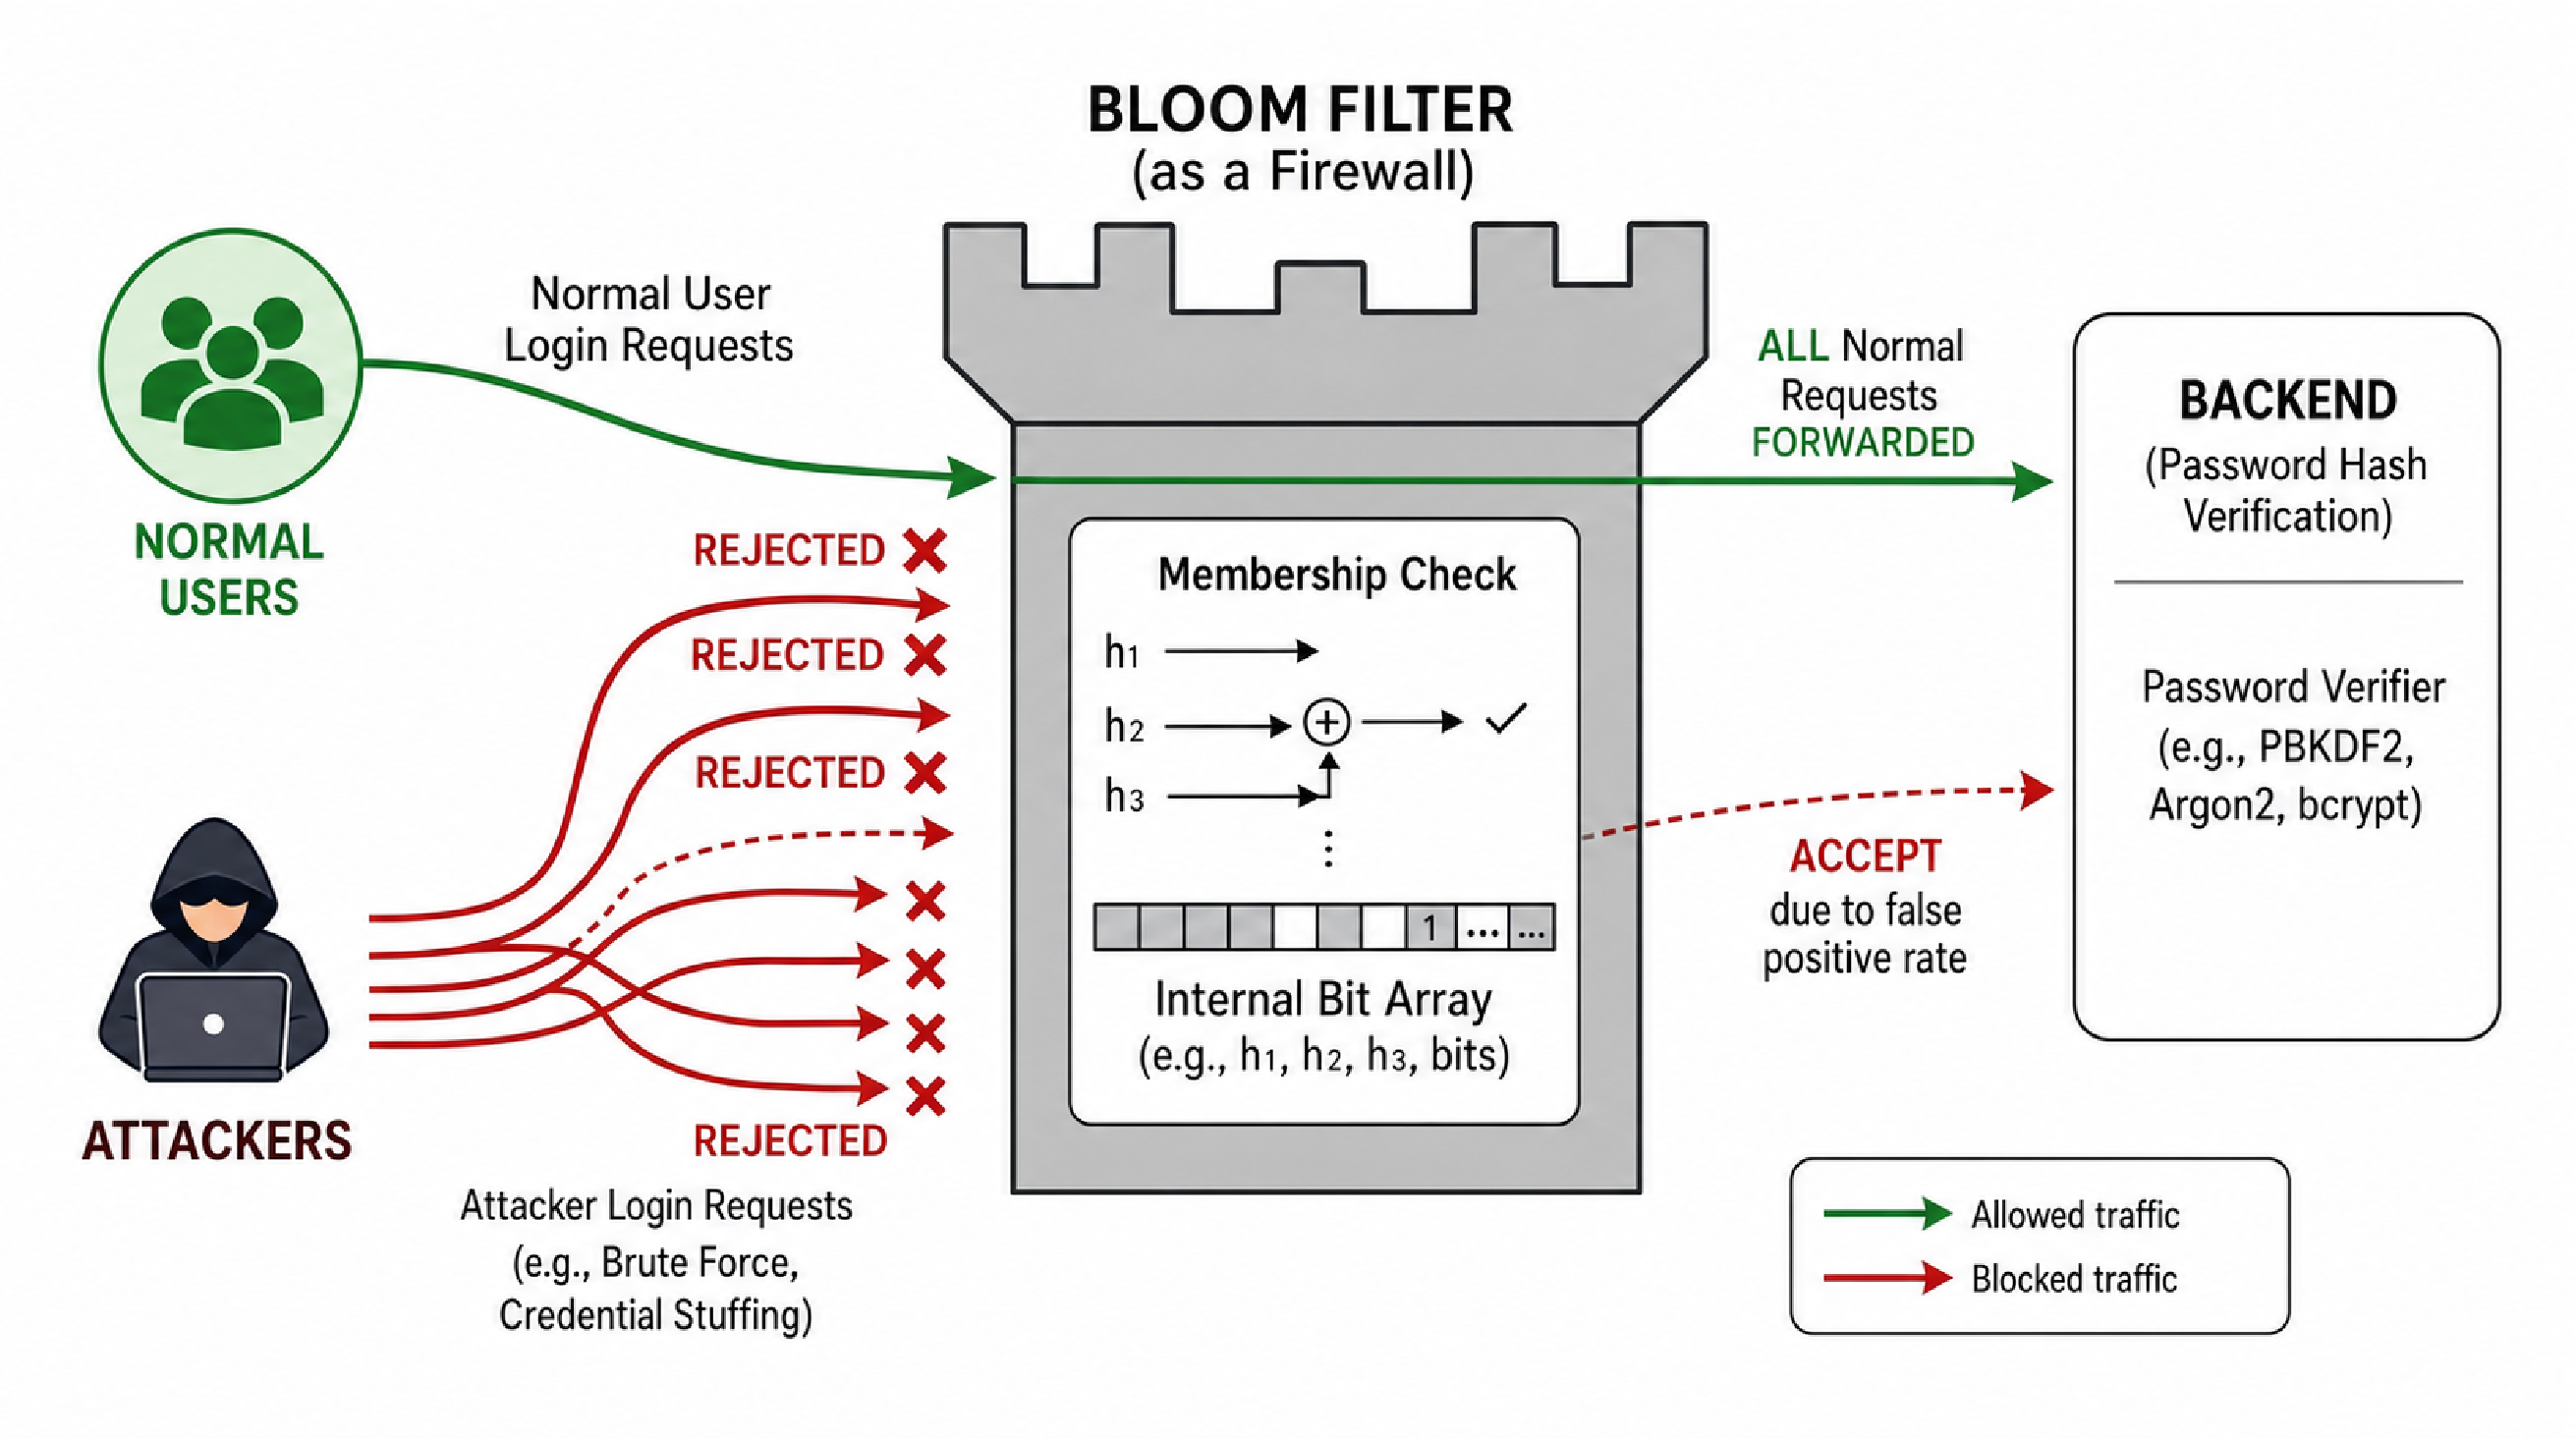
\includegraphics[width=\linewidth]{figure/LBF_pic/new_lbf_fig2.pdf}
  \caption{TRAPS as a one-sided admission-index layer before the password-verification backend.}
  \label{fig:systemoverview}
\end{figure}

TRAPS separates routing, indexing, and authentication. The learning and risk oracle selects a stable region for the submitted credential. The region-local substrate tests whether the corresponding trapdoor is represented. A positive result forwards the request to the backend; it does not authenticate the user. A negative result or replay-cache hit produces the same generic failure response as an ordinary backend reject.

\paragraph{Enrollment and rotation}
When a credential is created or rotated, the backend samples a salt \(s_u\), sets a password-version number \(v_u\), and stores the slow verifier \(H(pw,s_u)\). Registration-time policy may reject passwords using exact policy checks. If a credential is accepted but marked risky, for example due to known-password-list membership or chosen-password registration signals, TRAPS records a stable risk marker and inserts the credential trapdoor into a hardened region.

\paragraph{Login}
For a login attempt \((u,pw)\), the frontend obtains salt, stable metadata, and version from a read-only edge directory. Unknown usernames use a dummy tuple. TRAPS computes the region, derives the trapdoor, checks the replay-suppression cache, and queries the region-local substrate. Only positive, non-cached attempts reach the backend.

\paragraph{Stable route coverage}
For online context \(c\), let \(\Gamma_e(u,pw,c)\) be the set of epoch/region pairs that may contain the current represented credential under the deployment's routing contract. TRAPS may locally reject only after every substrate in \(\Gamma_e\) has been queried and returned negative. The evaluated \texttt{stable\_only} profile makes \(\Gamma_e\) a singleton by using credential- and epoch-stable features. A deployment that uses volatile context such as source, device, or time for region selection must either replicate the credential across all possible queried regions or fail-to-backend rather than AMQ-rejecting when coverage cannot be computed.

\paragraph{Backend feedback}
If the backend returns a definitive credential mismatch for a forwarded request, TRAPS records a replay token for that tuple. Subsequent submissions of the same invalid tuple are rejected before expensive verification.

\subsection{Threat Model}
\label{sec:threat-model}

We consider an online availability adversary whose goal is to maximize the number of incorrect attempts that reach the expensive backend. The adversary may choose usernames and passwords adaptively, distribute requests across many sources, use leaked or popular password lists, and infer from side effects that some invalid requests reached the backend.

The adversary knows the architecture, public algorithms, and broad feature families. Unless explicitly stated otherwise, it does not know epoch trapdoor keys, replay-cache keys, protected screening records, non-public stable metadata, or live indexing state. TRAPS does not rely on secrecy of the learned routing model; Section~\ref{sec:correctness-bound} gives the steering bound when per-region caps are enforced.

\paragraph{Known-password attack}
In a known-password attack, denoted \(\mathsf{KPwA}\), the adversary does not modify the active credential set during the attack window. It issues login attempts whose password distribution is concentrated on known weak, leaked, popular, policy-denied, or otherwise attacker-preferred passwords. Attempts that happen to be correct credentials are forwarded by design and are not counted as pre-screening failures.

Let \(U_j^{(\mathrm{K})}(T)\) be the number of distinct invalid credential tuples routed to region \(j\) during window \([0,T]\), after collapsing exact replays of the same tuple. The expected backend load from first-time invalid false forwards is
\[
\mathbb{E}
\left[
F_{\mathrm{adv}}^{(\mathrm{K})}(T)
\right]
=
\sum_{j=1}^{r}
U_j^{(\mathrm{K})}(T)\varepsilon_j.
\]

\paragraph{Chosen-password attack}
In a chosen-password attack, denoted \(\mathsf{CPwA}\), the adversary obtains bounded access to normal registration, password-reset, or password-rotation interfaces. Each successful operation creates or changes an attacker-controlled credential and causes a pre-verifier insertion. These operations are subject to the service's ordinary abuse controls and have non-negligible cost.

Let \(\Delta_j\) be the number of attacker-chosen accepted credentials inserted into region \(j\). If the occupancy of region \(j\) changes from \(N_j\) to
\[
N_j'=N_j+\Delta_j,
\]
then a subsequent invalid flood with \(U_j^{(\mathrm{C})}(T)\) distinct invalid tuples has expected residual backend load
\[
\mathbb{E}
\left[
F_{\mathrm{adv}}^{(\mathrm{C})}(T)
\right]
=
\sum_{j=1}^{r}
U_j^{(\mathrm{C})}(T)\varepsilon_j(N_j+\Delta_j).
\]
This models indexing-state poisoning and false-forward amplification. Successful logins using attacker-owned valid credentials remain ordinary valid traffic and are handled by complementary account-abuse controls.

\paragraph{Backend-overload objective}
Let \(C_{\mathrm{BE}}\) be the sustained backend capacity in full password verifications per unit time. Let \(L_{\mathrm{hon}}(T)\) be honest forwarded load and \(F_{\mathrm{adv}}(T)\) be attacker-induced false-forwarded load. The backend is overloaded if
\[
L_{\mathrm{hon}}(T)+F_{\mathrm{adv}}(T)\ge C_{\mathrm{BE}}T.
\]
TRAPS improves availability by reducing \(F_{\mathrm{adv}}(T)\) through region-specific residual budgets and replay suppression.

\paragraph{Out of scope}
TRAPS targets the password-verifier bottleneck under invalid-credential pressure. Attacks consisting solely of repeated logins using already-valid attacker-owned credentials are handled by complementary controls such as registration throttling, CAPTCHA, proof-of-work, payment or identity friction, per-account rate limits, and risk-based step-up authentication. Network-layer flooding, connection exhaustion, full compromise of the trusted first-party frontend, and post-compromise offline password cracking using exposed screening keys and indexing state are outside the core availability claim.

\paragraph{Username enumeration}
Unknown usernames follow a dummy-salt and dummy-metadata path, and local drops and backend rejects use the same generic failure response. TRAPS is designed not to introduce a semantic username-enumeration channel beyond that of the underlying service. Operational deployments should additionally equalize directory hit and miss behavior, avoid branch-specific errors, rate-limit repeated probes, and monitor timing distributions for distinguishers.

\paragraph{Deployment failure modes}
The one-sided guarantee is conditional on operational invariants rather than on the learned model. A stale edge directory can route a newly active credential before its trapdoor is represented, so activation must be atomic or fail-to-backend until backend-only verification is safe. Replay-cache entries must be exact, versioned, and inserted only after definitive backend mismatches; approximate negative caches or stale password-version entries can create false rejects. Migration crashes are handled by keeping the old epoch queryable until the new epoch is fully populated and durably activated. Stale Bloom bits after password rotation only increase false forwards and are removed by rebuild or dynamic AMQ maintenance. Trapdoor and replay keys are rotated by epoch with dual-query migration; key compromise or full frontend compromise is outside the core claim and requires emergency rebuild and backend-side abuse controls. Timing padding and dummy-directory behavior are required when username enumeration resistance is part of the deployment objective.

\section{TRAPS Construction}
\label{sec:construction}

This section gives the TRAPS construction for one active epoch and the region-allocation objective. Layering trade-offs, key rotation, and migration details follow the epoch-update discipline below.

\subsection{Epoch Policy}

Fix an active epoch \(e\). The epoch has a trapdoor key \(K_e^{\mathrm{td}}\), a replay-suppression key \(K_e^{\mathrm{neg}}\), and a runtime policy
\[
\Pi_e
=
\left(
\phi_e,
\mathcal{O}_e,
\{\tau_j\}_{j=0}^{r},
\{\mathcal I_{e,j}\}_{j=1}^{r},
\varepsilon_{\mathrm{cap}}
\right).
\]
Here \(\phi_e\) is the stable feature extractor, \(\mathcal{O}_e\) is the learning and risk oracle, \(\{\tau_j\}\) are routing thresholds, \(\mathcal I_{e,j}\) is the region-local indexing substrate, and \(\varepsilon_{\mathrm{cap}}\) is the configured per-region residual forwarding cap.

For a credential attempt \((u,pw)\) with salt and metadata \((s,\sigma)\), TRAPS computes
\[
\begin{aligned}
x &= \phi_e(u,pw,\sigma), &
z &= \mathcal{O}_e(x), &
t &= f_{K_e^{\mathrm{td}}}(h(u,pw,s)).
\end{aligned}
\]
The score \(z\) selects region
\[
j=\pi_e(u,pw,\sigma)
\iff
\tau_{j-1}\le z<\tau_j.
\]
Routing depends on stable risk features; membership depends on the trapdoor. This separation keeps learning outside the authentication-correctness path.

\subsection{Credential Creation and Rotation}

When a password is registered or rotated, the service first applies its ordinary account-abuse and password-policy controls. Exact hard-deny checks, such as mandatory registration-time password-policy rejection, occur before TRAPS insertion. If the credential is accepted, TRAPS records the stable metadata needed by the active epoch, including any risk markers produced by known-password-list probes or chosen-password registration detectors.

TRAPS then computes the credential trapdoor
\[
t_u=f_{K_e^{\mathrm{td}}}(h(u,pw,s_u))
\]
and inserts \(t_u\) into the region selected by \(\pi_e(u,pw,\sigma_u)\). A risky but accepted credential is not treated as invalid; it is represented in a hardened region. This is essential for one-sided correctness: correct future logins using that credential must still be forwarded to the backend.

A credential becomes active only after the backend verifier, edge-directory entry, protected screening record, and region insertion have committed. This atomic activation rule prevents a valid credential from reaching the login path before it is represented.

\subsection{Login Screening}

For a login attempt \((u,pw)\), the frontend obtains \((\hat{s},\hat{\sigma},\hat v)\) from the edge directory. If \(u\) is unknown, it substitutes a dummy tuple \((\bar{s},\bar{\sigma},\bar v)\). TRAPS computes the region \(j\), trapdoor \(t\), and replay token
\[
\eta
=
\operatorname{HMAC}_{K_e^{\mathrm{neg}}}
\left(
e \parallel \hat v \parallel u \parallel t
\right).
\]

If the exact replay-suppression cache contains \(\eta\), the attempt is rejected locally with the generic failure response. Otherwise, TRAPS queries \(\mathcal I_{e,j}\). A negative result is locally rejected. A positive result is forwarded to the backend verifier \(H\). If the backend returns a definitive credential mismatch, TRAPS inserts \(\eta\) into the replay-suppression cache.

This path has one-sided screening correctness under the deployment invariant stated below: every active valid credential must be represented in at least one active queried epoch under the same routing decision used for insertion.

\subsection{Correctness and Adaptive Work Bound}
\label{sec:correctness-bound}

\paragraph{Operational contract}
The one-sided result is enforced by five deployment invariants. P1, stable route coverage: every represented credential is inserted into every epoch/region pair in \(\Gamma_e(u,pw,c)\), the complete online coverage set that the router may query for the credential. P2, directory completeness: the active directory maps every represented credential to at least one live region/filter version. P3, atomic activation: a directory/filter version becomes visible only after all represented credentials for that version have been inserted. P4, versioned migration: rebuild queries check all old/new versions in which the credential may reside, and old versions retire only after coverage is complete. P5, replay-cache safety: cache entries are exact backend-confirmed invalid tuples scoped by account and credential version, and are invalidated on account creation, password change, or credential-version change before the tuple can become represented.

\begin{theorem}[One-sided pre-screening]
Under P1--P5, TRAPS may forward or reject invalid tuples, but it never locally rejects a login attempt using a represented active credential. During maintenance or recovery, forwarding to the backend or querying a complete safe version preserves this contract until the next epoch is fully active.
\end{theorem}

\begin{proof}[Proof sketch]
For a represented credential, enrollment or migration inserted the same trapdoor into the same region that login recomputes from stable metadata and the submitted password. The exact replay cache cannot contain the current-version valid tuple because replay tokens are inserted only after backend mismatch. The region-local substrate is one-sided for inserted items, so it returns positive. If multiple epochs are active, TRAPS forwards when any active epoch returns positive.
\end{proof}

\begin{theorem}[Replay-capped invalid work]
For a fixed epoch with exact replay retention, if every region satisfies \(\varepsilon_j\le \varepsilon_{\mathrm{cap}}\), then an adaptive adversary issuing a set \(\mathcal U_A\) of distinct invalid credential tuples causes expected backend work
\[
\mathbb{E}[W_A]
\le
\sum_{x\in\mathcal U_A}\varepsilon_{j(x)}
\le
|\mathcal U_A|\varepsilon_{\mathrm{cap}} .
\]
Repeated submissions of a backend-rejected false positive do not add backend work during the replay-token retention window.
\end{theorem}

Here \(W_A\) counts backend verifier invocations induced by invalid tuples. The theorem therefore gives the direct per-distinct-tuple backend-work bound \(\mathbb E[W_A]/|\mathcal U_A|\le\varepsilon_{\mathrm{cap}}\), with replay discoveries consuming at most one backend verification while retained.

\subsection{Known-password and Chosen-password Routing}

TRAPS treats known-password lists and chosen-password detectors as risk signals rather than login-time validity decisions.

For known-password traffic, a risk-list probe can route attempts using leaked, weak, popular, or policy-denied passwords into a hardened region with a lower residual forwarding budget. If the probe misses some risky attempts, those attempts remain in a less hardened region; correctness is unaffected. If the probe falsely marks an attempt as risky, the attempt receives stricter screening or step-up treatment, but TRAPS does not accept or reject a credential solely because of that approximate signal.

For chosen-password pressure, registration-side detectors can mark accepted credentials as CPwA-suspect. These credentials are inserted into a hardened region, increasing its occupancy but preserving their validity. The allocation rule below reserves memory for this occupancy pressure and enforces a per-region cap so that steering into the hardened region remains bounded.

Risk-list updates that would change the routing of already active valid credentials are deployed through the epoch mechanism in this section. In particular, a newly introduced password-derived risk predicate cannot be used to reroute legacy credentials unless the old region remains queried or the credentials have been migrated.

\subsection{Risk-aware Region Allocation}

Let \(M\) be the total memory budget and \(M_j\) the memory assigned to region \(j\). For the Bloom-filter instantiation, define
\[
\beta_{\mathrm{BF}}=(\ln 2)^2.
\]
For provisioned occupancy \(\bar N_j\), the region residual forwarding probability is approximated by
\[
\varepsilon_j(M_j;\bar N_j)
\approx
\exp
\left(
-\beta_{\mathrm{BF}}\frac{M_j}{\bar N_j}
\right).
\]

The risk oracle induces attack masses over regions. Let \(q_j^{(\mathrm{K})}\) denote the fraction of distinct known-password invalid attempts routed to region \(j\), and let \(\alpha_j\) denote the estimated chosen-password insertion pressure in region \(j\). TRAPS uses the risk weight
\[
a_j
=
q_j^{(\mathrm{K})}
+
\lambda_{\mathrm{C}}\alpha_j,
\]
where \(\lambda_{\mathrm{C}}\ge 0\) controls how aggressively the system reserves memory for chosen-password occupancy pressure.

TRAPS chooses region memory by solving
\[
\begin{aligned}
\min_{\{M_j\ge 0\}}\quad
&\sum_{j=1}^{r} a_j\varepsilon_j(M_j;\bar N_j)\\
\text{s.t.}\quad
&\sum_{j=1}^{r}M_j\le M,\\
&\varepsilon_j(M_j;\bar N_j)\le \varepsilon_{\mathrm{cap}}
\quad \forall j .
\end{aligned}
\]
The objective minimizes weighted residual false forwards, while the cap ensures that no region becomes an arbitrarily weak steering target.

\begin{theorem}[Capped water-filling allocation]
For nonempty Bloom-backed regions with \(\bar N_j>0\), the allocation problem is feasible iff
\[
M\ge B_\Sigma
:=
\sum_j
\frac{\bar N_j}{\beta_{\mathrm{BF}}}
\ln\frac{1}{\varepsilon_{\mathrm{cap}}}.
\]
When feasible, an optimal solution assigns \(M_j=B_j+m_j\), where \(B_j=(\bar N_j/\beta_{\mathrm{BF}})\ln(1/\varepsilon_{\mathrm{cap}})\). Zero-weight regions receive \(m_j=0\). For \(a_j>0\),
\[
m_j
=
\frac{\bar N_j}{\beta_{\mathrm{BF}}}
\left[
\ln
\frac{a_j\varepsilon_{\mathrm{cap}}\beta_{\mathrm{BF}}}
{\mu\bar N_j}
\right]_+ ,
\]
with water level \(\mu>0\) chosen so that \(\sum_j m_j=M-B_\Sigma\).
\end{theorem}

\begin{proof}[Proof sketch]
The cap is equivalent to the lower bound \(M_j\ge B_j\), giving the feasibility condition. After assigning the base memory, the residual problem minimizes the separable convex function \(\sum_j a_j\varepsilon_{\mathrm{cap}}\exp(-\beta_{\mathrm{BF}}m_j/\bar N_j)\) over a simplex. The KKT conditions are sufficient. Positive residual allocations equalize marginal residual-forward reduction, and inactive coordinates are clipped at zero, yielding the stated water-filling rule.
\end{proof}

This is the allocation step evaluated as TRAPS learned allocation in Section~\ref{sec:experiments}.

The same control-layer objective can be instantiated with exact keyed fingerprints by choosing region-specific tag lengths \(b_j\), with residual collision budget approximately \(2^{-b_j}\). The empirical implementation in this paper uses the Bloom-filter instantiation.

\subsection{Dynamic Capacity Adaptation}
\label{sec:dynamic-capacity}

The static allocation above applies to one epoch. In deployment, the attack mixture can change: KPwA traffic can shift across password populations, CPwA registrations can increase occupancy in selected regions, and replay-cache observations can reveal where residual false forwards occur. TRAPS therefore treats region capacities as epoch targets produced by a control-plane optimizer.

Let \(w\) index a control window. TRAPS maintains smoothed estimates of distinct invalid traffic, CPwA-suspect insertions, and backend-confirmed false forwards per region. It converts these observations into a protected occupancy target
\[
\bar N_{j,w}^{+}
=
N_{j,w}
+
s_{j,w}
+
\chi_{\mathrm C}\overline\Delta_{j,w},
\]
and a dynamic risk weight
\[
a_{j,w}
=
\omega_{\mathrm K,w}\widehat q_{j,w}^{(\mathrm K)}
+
\omega_{\mathrm C,w}\widehat q_{j,w}^{(\mathrm C)}
+
\lambda_{\mathrm C}\widehat\alpha_{j,w}
+
\lambda_{\mathrm R}\widehat r_{j,w}.
\]
Here \(N_{j,w}\) is current represented occupancy, \(s_{j,w}\) is a safety margin, \(\overline\Delta_{j,w}\) is smoothed CPwA-suspect insertion pressure, \(\widehat q_{j,w}^{(\mathrm K)}\) and \(\widehat q_{j,w}^{(\mathrm C)}\) are estimated invalid-query mixtures, \(\widehat\alpha_{j,w}\) is normalized insertion pressure, and \(\widehat r_{j,w}\) is the normalized replay-cache false-forward discovery rate.

The next-epoch target solves the capped allocation problem with \(\bar N_{j,w}^{+}\) and \(a_{j,w}\). Optionally, the optimizer adds a convex transition penalty to avoid unnecessary capacity churn. Capacity reductions are realized only through epoch rebuild and dual-query migration, because shrinking an active Bloom filter in place could violate one-sided correctness. If the cap is infeasible under the current memory budget and projected occupancy, the control plane must increase memory, slow further CPwA-suspect insertions, relax the cap in degraded mode, or combine these actions.

The main replay figures use frozen capacities selected from training/validation statistics. Section~\ref{sec:exp-index-microbench} separately evaluates a next-epoch dynamic-capacity and drift-guard policy using previous-window region observations only; the dynamic and fallback rows use no future labels.

\subsection{Epoch Updates}

TRAPS distinguishes routing-preserving updates from routing-changing updates. Routing-preserving changes, such as changing layer splits inside a fully populated region, can be activated after the affected structures have been populated.

Routing-changing updates are deployed as new epochs. If the new routing decision can be computed from protected screening records, the new epoch is rebuilt off path and dual-queried during migration. If the new routing decision requires password-derived information that was not recorded at enrollment, the old epoch remains active and the credential migrates lazily after successful authentication, password rotation, or account recovery.

This update discipline preserves the central invariant: every active valid credential is represented in at least one active queried epoch under the routing rule used for insertion.

\section{Experiments}
\label{sec:experiments}

Our evaluation addresses five questions: at fixed memory, how many invalid expensive point queries each admission index forwards (RQ1); how much learned region-wise AMQ allocation helps beyond global or handcrafted partitions (RQ2); how robust that benefit is under train/test shift, replay, and occupancy pressure (RQ3); how admission decisions translate into backend queueing and worker provisioning (RQ4); and whether public trace-conditioned arrival/account skew changes the conclusions (RQ5).

\subsection{Experimental Setup}

\begin{table}[t]
  \centering
  \footnotesize
  \caption{Backend verifier latency.}
  \label{tab:backend-benchmark}
  \begin{tabularx}{\columnwidth}{lXX}
    \toprule
    Metric & Argon2id & PBKDF2 \\
    \midrule
    Parameters
      & \(t=3\), \(m=65536\) KiB, \(p=1\)
      & iter.\(=600000\), hash\(=\texttt{SHA-256}\), dkLen\(=32\) B \\
    Verifier calls
      & 78,620
      & 78,620 \\
    Mean
      & 122.07 ms
      & 184.32 ms \\
    Median (P50)
      & 99.71 ms
      & 177.76 ms \\
    P95
      & 155.88 ms
      & 192.04 ms \\
    P99
      & 162.96 ms
      & 316.78 ms \\
    Single-worker cap.
      & 8.19 verif./s
      & 5.43 verif./s \\
    \bottomrule
  \end{tabularx}
\end{table}

\begin{table}[t]
\centering
\scriptsize
\setlength{\tabcolsep}{3pt}
\caption{Benign and attack workload model.}
\label{tab:workload-model}
\begin{tabular}{p{0.24\linewidth} p{0.66\linewidth}}
\toprule
\textbf{Item} & \textbf{Specification} \\
\midrule
\multicolumn{2}{l}{\textit{Benign workload}} \\
Horizon & 7 days \\
Session count & Poisson with bucket-specific \(\lambda\), scaled by weekday/weekend factors \\
Rate bucket & rare / weekly / daily / power \\
Session pattern & success / typo-success / old-password-success / new-device-success / benign-failure / repeat-success \\
Time & hourly weights: morning / afternoon / evening / night / mixed \\
Region & mostly home; occasional adjacent/far travel \\
Device & known-device pool; occasional new device \\
\midrule
\multicolumn{2}{l}{\textit{Attack workload}} \\
Credential stuffing & existing accounts; leaked current/old/wrong pairs; far region, attacker UA \\
Password spraying & broad accounts; top-\(k\) passwords; distributed attacker IPs \\
Brute force & small target set; repeated guesses; short bursts \\
Old-password replay & password-changed accounts; old password only; attacker-controlled metadata \\
Adaptive evasion & sampled accounts; mixed guesses; benign-like UA/device/region \\
Benign-mimic flood & broad high-volume accounts; mostly wrong guesses; benign-like metadata \\
Nonexistent-account flood & fake/mixed accounts; random/common guesses; mixed benign-like/attacker-like metadata \\
Low-and-slow distributed & many accounts; sparse guesses; wide IP pool, benign-like timing \\
Timing probe & repeated target variants; incorrect probes; metadata permutations \\
\bottomrule
\end{tabular}
\end{table}

\begin{table}[t]
\centering
\caption{Baselines and metrics.}
\footnotesize
\setlength{\tabcolsep}{2.5pt}
\renewcommand{\arraystretch}{0.94}
\begin{tabularx}{\columnwidth}{@{}p{0.82cm}p{1.95cm}X@{}}
\toprule
Type & Item & Description \\
\midrule
\multicolumn{3}{@{}l}{\textit{Baselines}} \\
Ext. & Backend only & No pre-screening; forwards all requests. \\
Ext. & Rate limit & Progressive throttling or lockout after failures~\cite{nist_sp800_63b_4_2025,owasp_authentication_cheat_sheet}. \\
Ext. & Blocklist & Registration-time or policy-side weak-password denylist screening~\cite{nist_sp800_63b_2017,nist_sp800_63b_4_2025,owasp_authentication_cheat_sheet}. \\
Ext. & Global Bloom & Single global Bloom filter over the same PRF trapdoors and total memory budget as TRAPS~\cite{Bloom1970BloomFilter,broder2004network}. \\
Diag. & Peppered tag & Exact keyed fast-verifier tag with uniform or adaptive tag lengths. \\
Diag. & Hash partition & Non-learned partitioned Bloom filter using hash/account partitions under the same total memory. \\
Diag. & Risk partition & Handcrafted-risk partition using known-password markers without a learned router. \\
Diag. & Neg. cache & Exact account-local cache of backend-confirmed invalid tuples. \\
Diag. & Oracle AMQ & Non-deployable allocation using held-out invalid-query masses. \\
Op. & Rate+tag & Token-bucket throttling plus peppered tags; may throttle valid requests. \\
Int. & TRAPS-Single & Risk-partitioned single-layer AMQ screening. \\
Int. & TRAPS-Layered & Risk-partitioned layered screening with early negative exits. \\
Int. & TRAPS-Strict & Stricter capped allocation policy; no login-time risk-only rejection. \\
\midrule
\multicolumn{3}{@{}l}{\textit{Metrics}} \\
Pri. & Valid-cred. FNR & Valid credentials rejected in error. \\
Pri. & Invalid fwd. rate & Invalid requests sent to the backend. \\
Pri. & Backend checks & Number of backend password verifications. \\
Aux. & Load reduction & Derived reduction in backend workload relative to no pre-screening. \\
Pri. & Login p95 latency & 95th-percentile latency of legitimate logins~\cite{dean2013tail}. \\
Aux. & Frontend mean cost & Mean compute cost of frontend screening. \\
Aux. & Memory footprint & Memory used by the screening layer. \\
Aux. & Backend time & Total backend verification time. \\
Aux. & Capture rate & Invalid requests blocked; complement of invalid forwarding rate. \\
\bottomrule
\end{tabularx}
\label{tab:baseline_metric_compact}
\end{table}

\paragraph{Configurations}
Experiments run on 64-bit Microsoft Windows~11 Pro 24H2 with a 13th Gen Intel Core i9-13900KF CPU and 16\,GB RAM. The Python~3.12 prototype uses optimized OpenSSL and Argon2 library backends, and all baselines and TRAPS variants share the same Argon2 and PBKDF2 parameters. Timing microbenchmarks use the Windows high-performance power plan and synchronous single-worker execution to calibrate per-attempt verifier cost, not production throughput. The reproducibility package\footnote{Anonymous artifact URL: \url{https://anonymous.4open.science/r/ICDETRAPS20260609}.} includes the workload generator, replay scripts, plotting scripts, and exported audit denominators.

\paragraph{Measurement modes}
We use five modes: a verifier-path benchmark for single-worker backend cost; replay evaluation over identical event streams; seeded production-baseline frontiers with denominators and confidence intervals; distribution-shift grids over target skew, risk drift, replay, and occupancy pressure; and method-specific bounded-worker queueing using the measured Argon2 service time.

\paragraph{Prototype and evaluation pipeline}
All methods share the same \texttt{verify\_password} interface and backend registry format; TRAPS changes only which attempts are forwarded. Each forwarded attempt therefore incurs the same backend path, including registry lookup, stored-hash parsing, salt and parameter recovery, password hashing, and constant-time comparison. Passwords are drawn from the \texttt{current\_password} field of \texttt{accounts.csv}, preserving the password-length distribution, and verification reads the complete stored hash from \texttt{backend\_registry.csv}. We calibrate forwarded-attempt cost with 78{,}620 single-worker verifier calls per backend configuration; the benchmark excludes network I/O, client load generation, queueing, frontend screening, and inter-request concurrency.

For auxiliary backend-work accounting, if a method forwards \(F\) attempts and the measured mean verifier cost is \(\bar{t}_{\mathrm{verify}}\), we compute
\[
W_{\mathrm{verify}} = F \cdot \bar{t}_{\mathrm{verify}} .
\]
Main method comparisons are based on forwarded attempts under the shared backend path; the benchmark only maps those attempts to an implementation-level cost scale.

\paragraph{Data preparation and label construction}
Credential-match inference is allowed only when credential evidence is user-unique or an explicit event-level validity label is present; otherwise, the match label remains unknown. A valid attempt is a labeled match to a represented active credential, and an invalid attempt is a labeled nonmatch; unknown attempts are excluded from false-reject and false-forward denominators. The represented set inserted into TRAPS comes from the active account snapshot for the epoch, while audit fields such as \texttt{credential\_valid}, \texttt{ground\_truth\_match}, \texttt{is\_attack}, \texttt{attack\_type}, and \texttt{campaign\_id} are retained for evaluation but excluded from the online-safe router feature set.

Zero-event replay counts are reported with finite-denominator context: we report the corresponding denominators and binomial confidence intervals, while correctness for represented credentials follows from the one-sided invariant in Section~\ref{sec:correctness-bound}. For each method we report both raw invalid-forward rate and first-seen invalid-forward rate. Replay caches should reduce only repeated invalid forwards; if a cache changes first-seen forwarding, the implementation is treated as invalid.

\paragraph{Time-causal feature extraction and feature eligibility}
The feature builder computes replay-time features in timestamp order, but the main deployment evaluation uses only a predeclared online-safe feature list with the conservative \texttt{stable\_only} profile. This profile excludes volatile history, delayed-feedback fields, labels, backend outcomes, raw credentials, hashes, salts, passthrough fields, model scores, future-looking fields, and audit-only columns; excluded time-causal history features remain available only for offline diagnostics and ablations.

\paragraph{Router training, calibration, and region construction}
TRAPS trains the learned component as a pre-screening router rather than a pure attack classifier. Represented valid attempts form the ordinary class, while known invalid and nonexistent-account attempts form the suspicious class; attack labels are retained for diagnostics and fallback supervision. We sort events by timestamp and use a chronological 70/15/15 train/validation/test split. Candidate routers are trained only on training data, calibrated on validation data with Platt scaling, and thresholded on validation data under a legitimate-intercept constraint.

TRAPS partitions the calibrated route-score space into a fixed number of regions using validation-score statistics. The resulting cut points are frozen before test evaluation. These region statistics drive the region-wise Bloom-filter allocation used by TRAPS variants; held-out test statistics are used only for reporting and auditing, not for fitting the router or selecting thresholds.

\paragraph{Allocation policy in the evaluation}
The default end-to-end figures use a single frozen epoch whose region capacities are selected from training and validation statistics. This isolates the effect of routing, partitioning, and allocation from feedback-loop effects. The shift-grid suite then evaluates dynamic-capacity control separately: previous-window region observations produce next-epoch capacity targets through rebuild or dual-query migration, without using future labels.

\paragraph{Workload construction}
The controlled generator is seeded by a cleaned public password lexicon derived from the RockYou wordlist.\footnote{Kali Linux packages the \texttt{wordlists} package, which contains \texttt{rockyou.txt}.} The lexicon supplies password-rank and weak-password distributions while the artifact stores only synthetic account records, PRF-based trapdoors, and generated verifier state. We deduplicate the lexicon and assign each candidate password a synthetic popularity score using a Zipf-like prior with adjustments for common weak-password patterns. From this prior, we instantiate 10{,}000 active accounts, sample current passwords by coarse strength segment, derive related old passwords through lightweight edits, and assign static account metadata from fixed distributions.

The generator then produces benign and adversarial authentication attempts over the same account universe. The benign stream includes valid logins and benign mistypes or password-reuse behavior, while the adversarial stream includes invalid credential attempts such as weak-password guessing, user/password spraying, reuse of old related passwords, and attempts against nonexistent or unrepresented accounts. These ingredients yield controlled, reproducible stress tests for the admission-index mechanisms. The benign and attack workload models are summarized in \autoref{tab:workload-model}.

\paragraph{Workload families}
We evaluate a disclosed workload matrix over target skew, replay fraction, risk drift, and occupancy injection. \emph{Credential-Flood Day} and \emph{Occupancy-Injection Attack} are named corners used for interpretability; aggregate frontiers, shift heatmaps, and worst-case tables report all grid cells. The named corners are grounded in Section~\ref{sec:threat-model}: the former fixes the active credential set while invalid attempts concentrate on leaked, weak, and reused passwords, and the latter adds attacker-controlled credential insertions before the login-flood window.

\paragraph{Baselines and metrics}
Table~\ref{tab:baseline_metric_compact} summarizes the baselines and metrics. Our main cryptographic pre-screening baseline is a single global Bloom filter over represented account--password trapdoors, denoted \emph{Global Bloom}. It uses the same represented credential set and the same total memory budget as TRAPS, but it does not use learned routing, score regions, or region-wise memory allocation. Improvements over this baseline isolate the value of routing, partitioning, and allocation rather than the value of using a Bloom pre-screener at all.

Section~\ref{sec:blocks} discusses exact keyed fingerprints as a compatible fast-verification substrate. The frontier includes uniform peppered tags, adaptive account-risk tags, exact negative caches, and rate-limit-plus-tag hybrids. These rows define the exact-fingerprint operating point; the AMQ rows define the approximate-membership operating point where TRAPS's allocation, cap, replay, and migration policies are exercised.

Let \(L\) be the set of represented valid attempts, \(I\) the set of invalid attempts, and \(F\) the number of attempts forwarded to the backend. Our primary safety metric is the valid-credential false negative rate, i.e., the fraction of represented valid attempts rejected before backend verification. Our primary load-shedding metric is the invalid forwarding rate, i.e., the fraction of invalid attempts that still reach the backend. We additionally report backend verification count, a backend-time proxy obtained by multiplying forwarded attempts by a shared verifier cost, and legitimate-request p95 latency. Frontend mean cost, memory footprint, capture rate, and backend-load reduction are reported as auxiliary metrics. Backend-load reduction is derived relative to the backend-only baseline.

\begin{figure}[t]
  \centering
  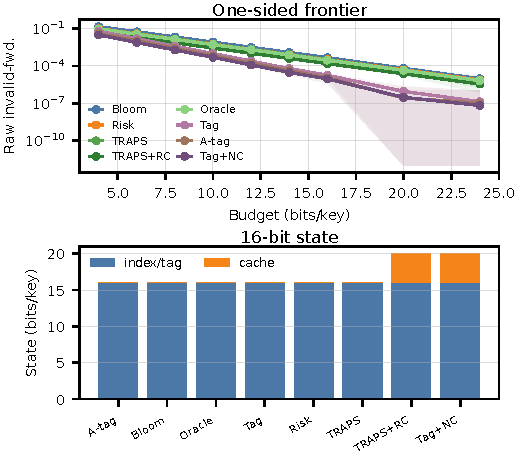
\includegraphics[width=\linewidth]{figure/icde_experiments/icde_frontier_production.pdf}
  \caption{Seeded admission-index frontier with production baselines.}
  \label{fig:icde-production-frontier}
\end{figure}

\subsection{Admission-Index Microbenchmarks}
\label{sec:exp-index-microbench}

\paragraph{Seeded production-baseline frontier}
Figure~\ref{fig:icde-production-frontier} compares admission-index baselines across 30 common-random-number seeds. Each seed uses 200k represented keys, 50k valid probes, and one million invalid probes; the reported data include raw and first-seen denominators, seed-level rates, 95\% intervals, and memory breakdowns. At 16 bits per represented key, Global Bloom forwards \(4.63\times10^{-4}\) of invalid probes on average. Handcrafted risk partitioning and TRAPS learned allocation reduce AMQ forwarding to \(3.21\times10^{-4}\) and \(3.06\times10^{-4}\), respectively; adding exact replay suppression lowers TRAPS's raw invalid-forward rate to \(1.55\times10^{-4}\) while preserving the same first-seen rate. The non-deployable oracle AMQ reaches \(2.90\times10^{-4}\), showing the remaining physical-design headroom.

Peppered fast tags give the exact-fingerprint frontier: observed uniform 16-bit tags forward \(1.78\times10^{-5}\), close to the \(2^{-16}\) calibration target, and adaptive account-risk tags forward \(1.09\times10^{-5}\). A production 64-bit tag bound is reported separately as a zero-event upper-bound row and is not plotted as part of the 16-bit frontier. The AMQ frontier answers a different physical-design question: given a one-sided approximate-membership frontend with residual false forwards, TRAPS allocates that residual channel across risk regions. The handcrafted risk row is a strong domain baseline with generator-aligned risk markers; the learned row tests automatic region discovery under the same capped AMQ allocation and replay machinery. Operational rate-limit-plus-tag hybrids reduce invalid forwards further but throttle valid requests, so they are reported separately from one-sided indexes.

\begin{figure}[t]
  \centering
  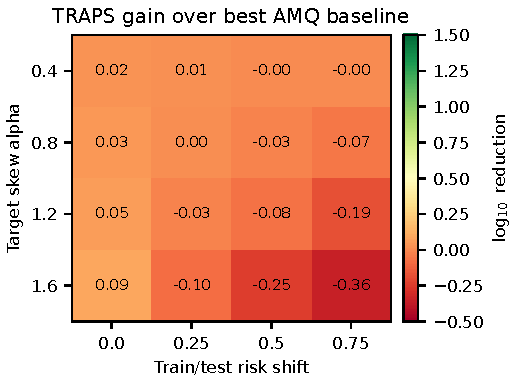
\includegraphics[width=\linewidth]{figure/icde_experiments/icde_shift_grid_heatmap.pdf}
  \caption{Distribution-shift grid. Cell values are median \(\log_{10}\) reduction of TRAPS over the best non-learned AMQ baseline; negative cells mark frozen-router degradation.}
  \label{fig:icde-shift-grid}
\end{figure}

\paragraph{Shift grid and worst cases}
Figure~\ref{fig:icde-shift-grid} sweeps target-account skew and train/test risk drift at 12 and 16 bits/key; separate exported sensitivity varies replay fraction and occupancy injection. TRAPS improves over non-learned AMQs when high-risk misses remain aligned with validation-time regions, and the grid also identifies when a frozen allocation should be refreshed. Table~\ref{tab:shift-dynamic} gives the 16-bit worst-case accounting: the worst frozen cell reaches \(1.51\times10^{-3}\), while previous-window next-epoch allocation and drift guard bring the worst case back near Global Bloom. Large drift is therefore a measured rebuild/fallback condition in the control plane.
The dynamic rows are the operational policy: frozen routing is the stale-state ablation, while next-epoch capacity and drift guard use only previous-window observations.

\begin{table}[t]
\centering
\caption{Shift/fallback accounting at 16 bits/key. Values are first-seen invalid-forward rates over 160 shift cells; dynamic rows use previous-window observations without future labels.}
\label{tab:shift-dynamic}
\scriptsize
\setlength{\tabcolsep}{3.3pt}
\begin{tabular}{lrrrr}
\toprule
Method & Median & P95 & Worst & Fallback cells \\
\midrule
Global Bloom & 4.59e-04 & 4.59e-04 & 4.59e-04 & 0 \\
Frozen TRAPS & 4.37e-04 & 1.00e-03 & 1.51e-03 & 0 \\
Dynamic next epoch & 3.76e-04 & 4.22e-04 & 4.36e-04 & 0 \\
Drift guard & 3.80e-04 & 4.58e-04 & 4.58e-04 & 20 \\
\bottomrule
\end{tabular}

\end{table}

\begin{figure*}[t]
  \centering
  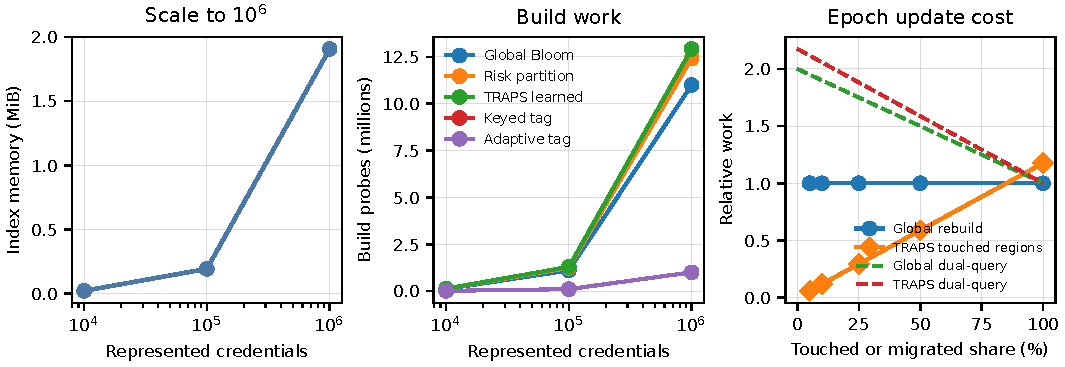
\includegraphics[width=\linewidth]{figure/icde_experiments/icde_scale_update_sweep.pdf}
  \caption{Scale and update behavior at 16 bits per represented credential.}
  \label{fig:icde-scale-update}
\end{figure*}

\paragraph{Scale and update cost}
Figure~\ref{fig:icde-scale-update} extends the index experiment to \(10^6\) represented credentials. At 16 bits per credential, the AMQ state is about 1.9 MiB for \(10^6\) entries before allocator metadata and replay-cache state. Build work scales linearly with represented credentials; the learned TRAPS allocation uses about 12.9 expected Bloom probes per invalid query at this budget, compared with 11 for a global Bloom filter and 1 for keyed tags. The update panel illustrates the operational value of regioning: routing-preserving updates that touch a subset of regions rebuild proportional state, while dual-query migration has a bounded transient probe multiplier that falls as credentials migrate.

\begin{figure*}[t]
  \centering
  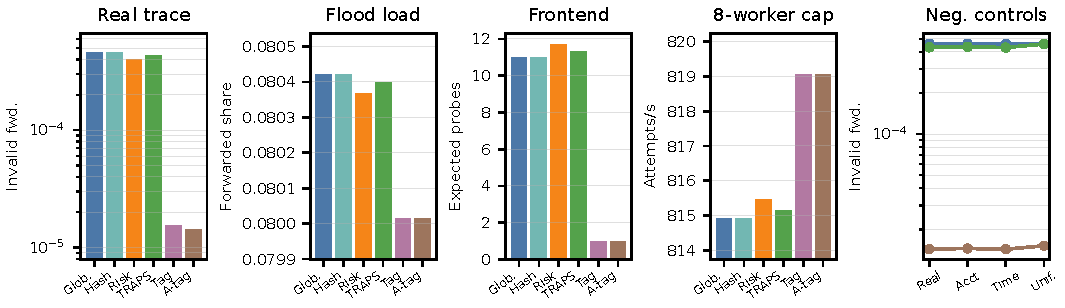
\includegraphics[width=\linewidth]{figure/icde_experiments/icde_lanl_trace_suite.pdf}
  \caption{LANL-conditioned routing/skew replay and router ablation.}
  \label{fig:icde-lanl-trace}
\end{figure*}

\subsection{Public Trace-Conditioned Replay}
\label{sec:exp-lanl}

\paragraph{LANL trace setup}
The public LANL authentication trace~\cite{Turcotte2018UnifiedHostNetwork} provides real enterprise arrival order, account/source skew, burstiness, routing-feature drift, and Success/Fail authentication status. The experiment samples 750{,}000 chronological events, uses the first 60\% for training, the next 20\% for validation, and the final 20\% for testing. The default full-stable token concatenates destination user, destination host, authentication type, logon type, and orientation. Source host, source user, status, and future fields are excluded from the token and router features. The exported denominator files report 8{,}702 destination users, 4{,}077 sources, top-1\% user event mass of 0.400, user-event Gini 0.753, and train/test token JS divergence 0.180.

\paragraph{Trace-conditioned baselines}
The LANL suite has two outcome views. First, a status-outcome replay uses the trace's real Success/Fail status as the event label. It yields 138{,}390 represented-success test events and 1{,}080 failure events; TRAPS learned routing forwards \(2.10\times10^{-7}\) of failures in expectation, versus \(4.59\times10^{-4}\) for Global Bloom and \(3.25\times10^{-4}\) for handcrafted risk partitioning, with zero represented-success false rejects. Second, an invalid-heavy stress replay uses the same LANL arrival/account/source skew with generated password-validity labels, yielding 7{,}015 represented-valid and 140{,}297 invalid test events. In that stress view, Global Bloom forwards \(4.59\times10^{-4}\), handcrafted risk partitioning \(3.98\times10^{-4}\), TRAPS learned routing \(4.32\times10^{-4}\), keyed tags \(1.53\times10^{-5}\), and adaptive tags \(1.44\times10^{-5}\). This split makes the trace result useful for both routing and substrate interpretation: the learned route extracts metadata signal in the status-outcome view, while the invalid-heavy view keeps a large denominator and shows exact tags as the fast-verifier frontier.

\paragraph{Learned-router ablation and sensitivity}
Account-shuffle, time-shuffle, and uniform-risk controls test whether routing uses enterprise metadata skew rather than future labels. Destroying risk information moves TRAPS back to the global Bloom rate. The status-outcome replay supplies real trace outcomes, while the invalid-heavy stress replay keeps the credential-flood denominator large enough to compare AMQ allocation policies.

\subsection{Named Workload Corners}
\label{sec:exp-corners}

The full grid carries the main evidence; the named KPwA/CPwA workloads provide interpretable corners. In the fixed-credential \emph{Credential-Flood Day} corner, TRAPS preserves the one-sided invariant and reduces invalid forwarding relative to the same-memory Global Bloom baseline when the learned regions match the attack skew. In the \emph{Occupancy-Injection Attack} corner, attacker-controlled insertions stress region capacity; the shift grid and ablation table expose the corresponding cap and refresh behavior across all cells.

\subsection{Ablation Study}
\label{sec:exp-ablation}

We next isolate learned partitioning, region-wise allocation, replay suppression, and capped allocation.

\begin{table}[t]
  \centering
  \scriptsize
  \caption{Mechanism ablation at 16 bits/key over 30 seeds.}
  \label{tab:traps-ablation}
  \begin{tabular}{lrrrr}
\toprule
Variant & Raw IFFR & First-seen IFFR & Backend calls & Cap viol. \\
\midrule
Full & 1.56e-04 & 3.12e-04 & 50156 & 0 \\
Hash router & 4.59e-04 & 4.59e-04 & 50452 & 0 \\
Equal alloc. & 4.59e-04 & 4.59e-04 & 50460 & 0 \\
No cap & 1.32e-04 & 2.65e-04 & 50136 & 2 \\
No replay & 3.12e-04 & 3.12e-04 & 50312 & 0 \\
Oracle & 1.48e-04 & 2.96e-04 & 50146 & 0 \\
\bottomrule
\end{tabular}

\end{table}

Table~\ref{tab:traps-ablation} separates raw invalid forwards from first-seen invalid forwards. Removing the learned router or region-wise allocation returns the AMQ close to the global Bloom rate. Removing replay suppression leaves the first-seen rate unchanged but doubles raw invalid forwards under a 50\% replay fraction, which is the expected behavior for an exact negative cache. The no-cap row can improve the median rate but creates cap violations, so it is not a safe deployment policy.

The main paper focuses on the ablation rows that directly test the ICDE claim: learned routing, allocation, replay suppression, and cap enforcement.

\begin{figure}[t]
  \centering
  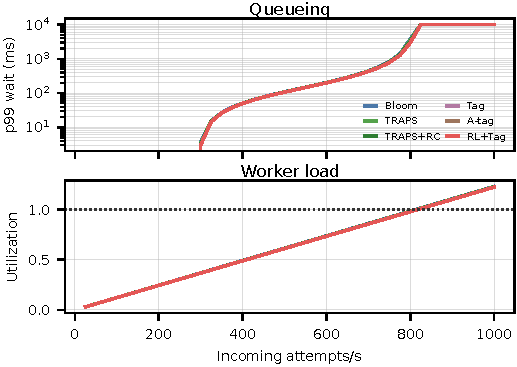
\includegraphics[width=\linewidth]{figure/icde_experiments/icde_queueing_by_method.pdf}
  \caption{Method-specific bounded-worker queueing with measured Argon2 service time.}
  \label{fig:icde-queueing}
\end{figure}

\subsection{Backend Saturation and Replay State}
\label{sec:exp-queueing-replay}

\paragraph{Bounded-worker queueing}
Figure~\ref{fig:icde-queueing} maps method-specific forwarding rates from the production frontier to backend-worker pressure using the 122.07 ms Argon2 mean service time and eight backend workers. With an 8\% valid-attempt fraction, all one-sided indexes keep utilization close because valid attempts dominate residual backend work; rate-limit hybrids are plotted with their measured valid-drop caveat rather than mixed into the one-sided frontier.
The queueing panel translates forwarding-rate deltas into worker provisioning and latency headroom under the shared backend service-time model.

\begin{figure}[t]
  \centering
  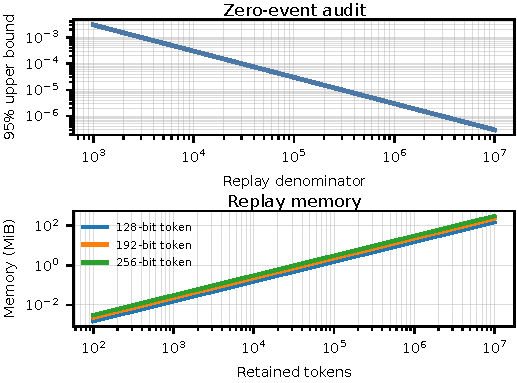
\includegraphics[width=\linewidth]{figure/icde_experiments/icde_replay_cache_ci.pdf}
  \caption{Replay-cache memory and finite zero-event audits.}
  \label{fig:icde-replay-cache}
\end{figure}

\paragraph{Replay cache and zero-event audits}
Figure~\ref{fig:icde-replay-cache} summarizes finite-audit and replay-state accounting. Zero events over \(10^5\) trials gives a 95\% upper bound of about \(3.0\times10^{-5}\), while retaining \(10^6\) backend-confirmed invalid tuples costs about 15.3 MiB with 128-bit tokens and 30.5 MiB with 256-bit tokens before hash-table overhead.

\subsection{Discussion and Limitations}
\label{sec:exp-limitations}

TRAPS reduces calibrated backend verification work while preserving zero observed pre-screening false rejects in the evaluated replays. The gains come from different layers: exact keyed tags define the strongest account-local fast-verifier frontier, while AMQ-backed TRAPS contributes capped residual-channel allocation, replay suppression, and migration-safe capacity control. The controlled generator keeps the KPwA and CPwA stress tests reproducible and varies attack skew, insertion pressure, and queueing load in isolation.

The end-to-end figures use a frozen epoch allocation selected from training and validation statistics. Section~\ref{sec:dynamic-capacity} specifies next-epoch capacity adjustment under changing KPwA mixtures, CPwA insertion pressure, and replay-cache discoveries; the scale/update experiment shows how rebuild and dual-query costs grow with represented credentials and touched regions.

The empirical adversary is the partial-information attacker from our threat model: it does not observe exact region assignments, thresholds, live filter state, or local drop decisions. With per-region caps, Section~\ref{sec:correctness-bound} bounds expected backend work per distinct invalid tuple by \(\varepsilon_{\mathrm{cap}}\), complementing robust-Bloom-filter notions~\cite{Naor2015AdversarialBF,NaorOved2022BetOrPass,LotanNaor2025MonotonicityBetting,Tirmazi2025PrivacyModelBF} with backend-work accounting and exact replay retention.

Production deployments integrate the admission index with concurrency control, queueing, latency padding, monitoring, abuse-response policy, and rebuild scheduling. The no-false-reject property relies on stable routing, atomic insertion, and versioned dual-query rebuilds; stale Bloom-filter bits from password changes are handled through periodic rebuilds or dynamic AMQ variants. TRAPS assumes a trusted first-party frontend, which matches the intended placement before the service's own password verifier.

\section{Related Work}
\label{sec:related-work}

\paragraph{AMQs and learned filters}
Bloom filters provide compact one-sided approximate membership with tunable false-positive probability~\cite{Bloom1970BloomFilter,broder2004network}; blocked, scalable, dynamic, Cuckoo, Xor, and Binary Fuse filters improve space or speed in different regimes~\cite{Putze2007BlockedBF,almeida2007scalable,Guo2006DynamicBloom,Fan2014CuckooFilter,Lemire2020XorFilter,Lemire2022BinaryFuse}. Learned indexes and learned Bloom filters use models to reduce space by predicting membership~\cite{Kraska2018LearnedIndex,Mitzenmacher2018NeurIPS}, with sandwiching and partitioning improving backup-filter trade-offs~\cite{Mitzenmacher2018NeurIPS,sato2023fast}. TRAPS uses Bloom filters for their simple one-sided semantics, but its learned component is only a stable router: membership remains a keyed trapdoor check, so model errors cannot create an accept path.

\paragraph{Adversarial and online indexing}
Classical Bloom-filter analysis assumes query independence. Robust Bloom filters, Bet-or-Pass, monotonicity/betting definitions, privacy-oriented models, and adversary-resilient learned Bloom filters study adaptive query selection~\cite{Naor2015AdversarialBF,NaorOved2022BetOrPass,LotanNaor2025MonotonicityBetting,Tirmazi2025PrivacyModelBF,Bishop2024AdversaryResilientLBF}. TRAPS is complementary: exact replay suppression prevents repeated exploitation of discovered false positives, and per-region caps bound expected backend work per distinct invalid tuple. The system also echoes resource-aware admission control, load shedding, and online index maintenance, but the login front end must preserve one-sided semantics for represented valid credentials during epoch rebuilds and dual-query migration.

\paragraph{Authentication and availability defenses}
Privacy Pass and OPRFs support privacy-preserving authorization and PRF evaluation~\cite{RFC9576PPArch,RFC9577PPAuth,RFC9578PPIssuance,RFC9497OPRF}; breach alerting, k-anonymity, PSI, PIR, and OPRF-based services check password exposure with limited leakage~\cite{Thomas2019PasswordCheckup,Cloudflare2018KAnonHIBP,ChaseMiao2020PSIInternet,PaXoS2020,Lin2025UnbalancedPSI}. Separately, application-layer availability defenses include rate limiting, scheduling, proof-of-work, CAPTCHA, and network filtering~\cite{zargar2013survey,Dwork1992Pricing,vonAhn2003CAPTCHA,Ranjan2006DDoSResilientSched,Ranjan2009DDoSShield,Srivatsa2008AdmissionControlWeb}. TRAPS sits at a narrower first-party bottleneck: it reduces password-hashing work under invalid credential floods while preserving pass-through for represented valid credentials.

\section{Conclusion}

TRAPS frames expensive password verification as a risk-aware one-sided admission-index physical-design problem. Learning supplies stable resource routing; keyed region-local substrates decide forwarding; the backend remains the accepting component. Across seeded frontiers, LANL status-outcome replay, invalid-heavy trace-conditioned stress, dynamic shift guards, update analysis, and bounded-worker queueing, the substrate frontier is clear: exact keyed tags give the strongest fast-verifier operating point, while AMQ-backed TRAPS provides capped allocation, replay suppression, and migration discipline for approximate-membership frontends. Under drift, previous-window monitoring drives next-epoch rebuild or fallback, turning learned routing into a managed control-plane component.


\section*{AI-Generated Content Acknowledgement}
The authors used OpenAI ChatGPT/Codex to assist with language editing, source-file inspection, reproducibility-script development, artifact packaging, and code-review suggestions. The authors reviewed and verified the resulting manuscript, experiments, code, figures, and claims, and remain responsible for the paper, artifact, and presentation.
\bibliographystyle{IEEEtran}
\bibliography{references}
\end{document}
